\documentclass[tikz,border=2mm]{standalone}
\usepackage{helvet}
\renewcommand{\familydefault}{\sfdefault}
\usetikzlibrary{arrows.meta,positioning}
\definecolor{datablue}{HTML}{4477AA}
\definecolor{methodgreen}{HTML}{228833}
\definecolor{modelorange}{HTML}{EE7733}
\definecolor{impactpurple}{HTML}{AA3377}
\begin{document}
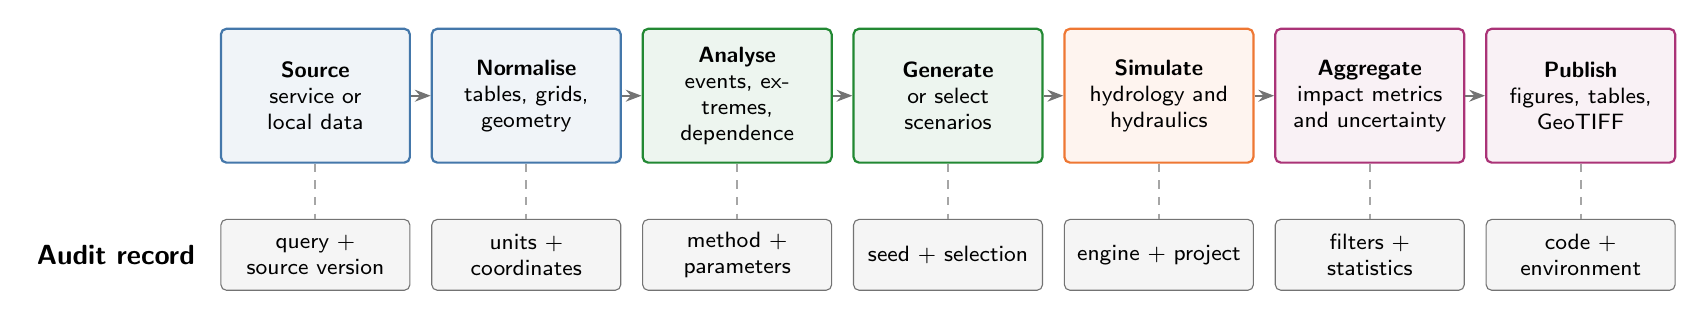
\begin{tikzpicture}[
  font=\fontsize{8}{9.4}\selectfont,
  stage/.style={rounded corners=2pt, line width=0.8pt, align=center,
    minimum width=24mm, minimum height=17mm, text width=21mm, inner sep=1.5mm},
  record/.style={rounded corners=2pt, draw=black!55, fill=black!4,
    align=center, minimum width=24mm, minimum height=9mm, text width=21mm,
    inner sep=1mm},
  arrow/.style={-{Stealth[length=2mm]}, line width=0.85pt, draw=black!55},
  link/.style={line width=0.7pt, draw=black!35, dashed}
]
\node[stage, draw=datablue, fill=datablue!8] (source) {\textbf{Source}\\service or local data};
\node[stage, draw=datablue, fill=datablue!8, right=2.5mm of source] (normal) {\textbf{Normalise}\\tables, grids, geometry};
\node[stage, draw=methodgreen, fill=methodgreen!8, right=2.5mm of normal] (events) {\textbf{Analyse}\\events, extremes, dependence};
\node[stage, draw=methodgreen, fill=methodgreen!8, right=2.5mm of events] (scenarios) {\textbf{Generate}\\or select scenarios};
\node[stage, draw=modelorange, fill=modelorange!8, right=2.5mm of scenarios] (simulate) {\textbf{Simulate}\\hydrology and hydraulics};
\node[stage, draw=impactpurple, fill=impactpurple!7, right=2.5mm of simulate] (impact) {\textbf{Aggregate}\\impact metrics and uncertainty};
\node[stage, draw=impactpurple, fill=impactpurple!7, right=2.5mm of impact] (product) {\textbf{Publish}\\figures, tables, GeoTIFF};

\draw[arrow] (source) -- (normal);
\draw[arrow] (normal) -- (events);
\draw[arrow] (events) -- (scenarios);
\draw[arrow] (scenarios) -- (simulate);
\draw[arrow] (simulate) -- (impact);
\draw[arrow] (impact) -- (product);

\node[record, below=7mm of source] (r1) {query + source version};
\node[record, below=7mm of normal] (r2) {units + coordinates};
\node[record, below=7mm of events] (r3) {method + parameters};
\node[record, below=7mm of scenarios] (r4) {seed + selection};
\node[record, below=7mm of simulate] (r5) {engine + project};
\node[record, below=7mm of impact] (r6) {filters + statistics};
\node[record, below=7mm of product] (r7) {code + environment};
\foreach \a/\b in {source/r1,normal/r2,events/r3,scenarios/r4,simulate/r5,impact/r6,product/r7}
  \draw[link] (\a.south) -- (\b.north);
\node[font=\bfseries, anchor=east] at ([xshift=-2mm]r1.west) {Audit record};
\end{tikzpicture}
\end{document}
